\chapter{Erarbeitung des Konzepts}\label{ch:conception}
Bevor mit der eigentlichen Implementierung begonnen werden kann wird ein grober Plan erstellt.
In diesem Plan beziehungsweise Konzept wird die Art und Weise definiert, wie die Anwendung funktionieren soll und gegebenenfalls werden UI-Prototypen erstellt.\pbreak%
%
Dieses Kapitel wird im Allgemeinen in die drei Hauptbereiche der Anwendung unterteilt, in denen die Ideen der Funktionsweise erklärt werden.
Dazu gehört das Erstellen und Verwalten von Projekten, das Bearbeiten und Zeichnen der eigentlichen Kartendaten und das Exportieren eines fertigen Projektes in das \acl{imdf}.
Diesen drei Abschnitten ist das Design-Konzept vorangestellt, in dem die Grundlagen für das Design der Benutzeroberfläche beschrieben werden.\pbreak%
%
Nach einigen Überlegungen und verschiedenen Arbeitstiteln wurde sich für den Anwendungsnamen \textbf{Indoor Architect} entschieden.
Somit wird in den folgenden Abschnitten mit Indoor Architect die Anwendung gemeint.

\section{Design-Konzept}
In diesem Abschnitt werden die allgemeinen Fragen bezüglich des Designs von Indoor Architect beschrieben.
Dabei wird genauer auf die Navigation durch die Anwendung eingegangen.
Im Anschluss wird vor allem die Trennung des Kartenbereichs von dem Rest der Anwendung genauer erklärt und die gewählten Farben dargestellt.\pbreak%
%
Anders als bei den analysierten aktuellen Lösungen aus \autoref{ch:analysis} soll Indoor Architect so minimalistisch wie möglich werden.
Trotzdem sollen alle wichtige Funktionen zur Erstellung von Indoor Maps enthalten bleiben.
Der Benutzer darf sich nicht in einem Projekt gefangen fühlen und sollte zu jeder Zeit ohne großen Aufwand zwischen verschiedenen Projekt wechseln können.

\subsection{Navigation}
Die Navigation durch die Anwendung wird mittels Push- und Pop-Navigation erreicht.
Dabei gibt es eine Hauptansicht, von der man in verschiedene Unteransichten navigieren kann und ebenso wieder zurück navigieren kann.
Der Vorteil gegenüber anderen Arten der Navigtion ist, dass es nur einen Pfad zu jeder Ansicht gibt und man daher besser im Blick behalten kann wo man sich befindet.
%
Um dem vorher beschreibenen Punkt gerecht zu werden, dass man schnell und einfach zwischen verschiedenen Projekten wechseln können sollte, wird eine Seitenleiste vorhanden sein.
In dieser Seitenleiste werden die Projekte und gegebenenfalls weitere Punkte aufgelistet, über die man einen anderen Kontext öffnen kann.
\begin{figure}[h!]
	\centering
	\vspace{15pt}
	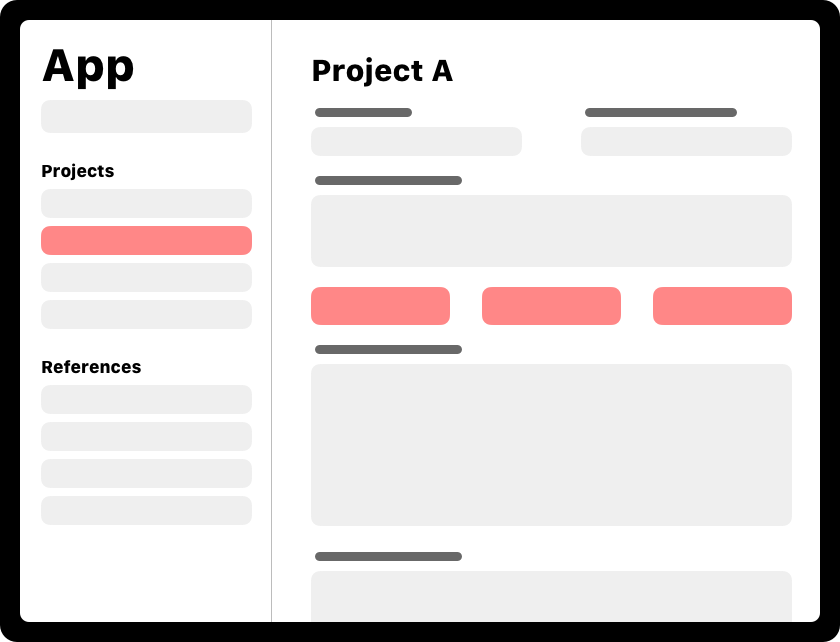
\includegraphics[scale=0.4]{images/design-app}
	\caption{Mockup der Hauptansicht eines Projektes}
	\label{fig:design-app}
\end{figure}
In der Abbildung \ref{fig:design-app} erkennt man, dass in der Seitenleiste auf der linken Seite das zweite Projekt (Project A) ausgewählt ist und auf der rechten Seite die Projektübersicht dargestellt wird.
Auf der rechten Seite kann der Benutzer nun das Projekt verwalten und Unteransichten öffnen, die in dem rechten Bereich angezeigt werden.
Die Seitenleiste bleibt weiterhin sichtbar, sodass globale Funktionen der Anwendung – wie die Einstellungen, das Durchsuchen der Anwendung oder das Erstellen eines neuen Projektes – zu jeder Zeit zugänglich sind.
Selbst wenn der Benutzer sich in tieferen Ebenen der Projekteinstellungen wiederfindet ist ihm stets klar in welchem Projekt er gerade navigiert.

\subsection{Trennung des Kartenbereichs}
Eine Ausnahme dabei ist der Kartenbereich.
Wenn ein Benutzer die Kartendaten eines Projektes bearbeiten möchte, muss der Karteneditor geöffnet werden.
Da für das Bearbeiten der Kartendaten eine möglichst große Fläche von Vorteil ist, wurde sich dazu entschieden dem Karteneditor den kompletten Bildschirm bereitzustellen.
Dem Benutzer wird dann nur der Kartenkontext angezeigt, sodass er sich auf diesen Bereich konzentrieren kann.
In der Abbildung \ref{fig:design-map} findet man in der oberen linken Ecke einen Schließen-Button, welcher den Karteneditor wieder schließt und den Benutzer zurück zur Projektübersicht bringt.
\begin{figure}[h!]
	\centering
	\vspace{15pt}
	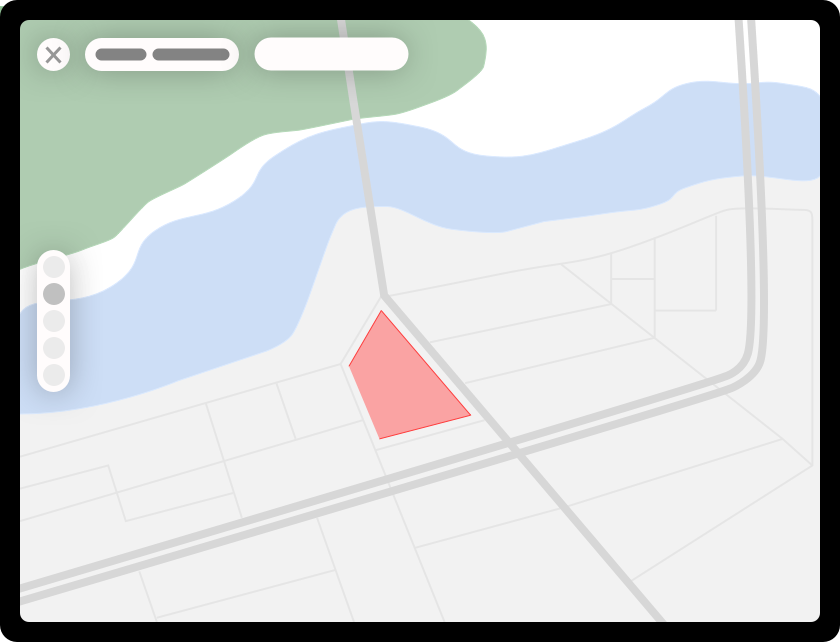
\includegraphics[scale=0.4]{images/design-map}
	\caption{Mockup der Kartenansicht eines Projektes}
	\label{fig:design-map}
\end{figure}

\subsection{Barrierefreiheit}
Für die Entwicklung von Indoor Architect ist es wichtig, dass auf die Barrierefreiheit geachtet wird.
Dies bedeutet unter anderem auf entsprechend hohe Kontrastwerte zwischen den verwendeten Farben zu achten und die Schriftgrößen richtig zu wählen.
Um die Ziele der Barrierefreiheit zu erreichen, kann man die bereits vorhandenen Schnittstellen des genutzten \Gls{sdk} verwenden.\pbreak%
%
Anstatt für einen Text eine Schriftart und Schriftgröße zu wählen, wählt man eine semantische Kategorie für den Textbereich (zum Beispiel \emph{Überschrift} oder \emph{Fließtext}).
Der Benutzer, welcher Funktionen der Barrierefreiheit nutzt und in seinen Geräteeinstellungen zum Beispiel eine größere Schrift eingestellt hat, wird auch in der Anwendung eine für ihn ansprechende Schrift wiederfinden anstatt die festgelegte Schriftgröße.
Ebenso kann das System die Schriftstärke je nach Präferenz des Benutzers wählen, wenn man dynamische Schriften erlaubt und die Stärke nicht manuell setzt.\pbreak%
%
Gleiches gilt für die Verwendung von Farben.
Wenn in Indoor Architect Farben verwendet werden, dann müssen diese aus vier unterschiedlichen Farben bestehen.
Zum Einen lässt sich zwischen einem hellen und einem dunklen Modus wechseln, zum Anderen gibt es für Benutzer mit Sehschwächen in den Geräteeinstellungen die Möglichkeit eine \emph{High Contrast}-Einstellung zu wählen.
Damit Indoor Architect diese Funktion der Barrierefreiheit unterstützen kann, muss für jede Farbe auch immer eine \emph{High Contrast}-Variante bereitsgestellt werden.
Daraus ergeben sich folgende vier Kombinationen pro Farbe:
\begin{itemize}
	\setlength\itemsep{0pt}
	\item[] \colorbox{redL}{\color{white}\texttt{\#ff3b30}\hspace{20pt}} \hspace{10pt}Normaler Kontrast
	\item[] \colorbox{redDL}{\color{white}\texttt{\#ff453a}\hspace{20pt}} \hspace{10pt}Dunkelmodus, Normaler Kontrast
	\item[] \colorbox{redH}{\color{white}\texttt{\#d70015}\hspace{20pt}} \hspace{10pt}Hoher Kontrast
	\item[] \colorbox{redDH}{\color{white}\texttt{\#ff6961}\hspace{20pt}} \hspace{10pt}Dunkelmodus, Hoher Kontrast
\end{itemize}
Die dargestellten Farbkombinationen sind die der vom System bereitgestellten Farbe Rot (\texttt{systemRed}).
Je nach Geräteeinstellung des Benutzers wird die entsprechende Farbe für den normalen oder den Hochkontrastmodus gewählt und angezeigt.\pbreak%
%
Neben der automatischen Anpassung der dargestellten Schrift und Farben gibt es noch weitere Möglichkeiten, wie die Barrierefreiheit für Benutzer verbessert werden kann.
Ein weiterer Schritt könnte das Vermeiden von Transparenzen und Animationen sein.
In den \emph{Human Interface Guidelines} für iOS-Anwendungen, welche Empfehlungen und Ressourcen für das UI-Design auf Apple-Plattformen bereitstellen, weist Apple darauf hin, dass Transparenzen und Animationen für einige Personen ablenkend oder sogar unangenehm sein können \parencite{APP2020a}.
Da keine starken Transparenzen in Indoor Architect eingebaut werden und die Animationen, die verwendet weden, bereits auf Barrierefreiheit achten, müssen dafür keine Schritte vorgenommen werden.
Für Benutzer die an Blindheit leiden gibt es zudem noch die \emph{VoiceOver}-Funktion, welche berührten Fließtext sowie unter anderem den Titel von Buttons vorließt.
Um die Aktion hinter dem Button auszuführen muss ein zweites mal auf den Button geklickt werden.
Auch in diesem Fall kann diese Barrierefreiheitfunktion außer acht gelassen werden, da die Betroffenen nicht Zielgruppe der Anwendung sind.
Selbst mit den entsprechenden Funktionen der Barrierefreiheit ist das Zeichnen auf den Kartendaten mit einer Blindheit in dieser Anwendung schwer zu verwirklichen.

\section{Erstellen von Projekten}
Das Erstellen eines Projektes sollte möglichst einfach und ohne großen Aufwand erfolgen.
Aus diesem Grund wird es ähnlich dem Auswählen von existierenden Projekten auch in der Sidebar die Möglichkeit geben ein Projekt zu erstellen.
Es muss lediglich ein Plus-Symbol geklickt werden und der Anwender kann die Grundinformationen für das Projekt eingeben.
Da das Erstellen eines Projektes nur ein kleiner Schritt ist und der Anwender nicht eine komplett neue Ansicht bekommen muss, wird das Formular als \emph{Popover} angezeigt.
Ein Popover ist eine Ansicht, die über den aktuellen Inhalt gelegt wird, welcher verdunkelt wird.
In der Abbildung \ref{fig:design-project-create} kann man erkennen, dass der Fokus auf das neue Formular gelegt wird, obwohl die Projektübersicht im Hintergrund weiter sichtbar ist.
Sobald der Anwender die Erstellung des Projektes bestätigt, wird er zu der Projektübersicht des neuen Projektes weitergeleitet.
Das Formular zur Erstellung bietet die Möglichkeit, drei Felder auszufüllen:
\emph{Projekttitel}, \emph{Projektkunde} und \emph{Projektbeschreibung}, von denen nur der Projekttitel ein Pflichtfeld ist.
Alle drei Felder können nach der Erstellung beliebig oft bearbeitet werden.
\newpage
\begin{figure}[h!]
	\centering
	\vspace{15pt}
	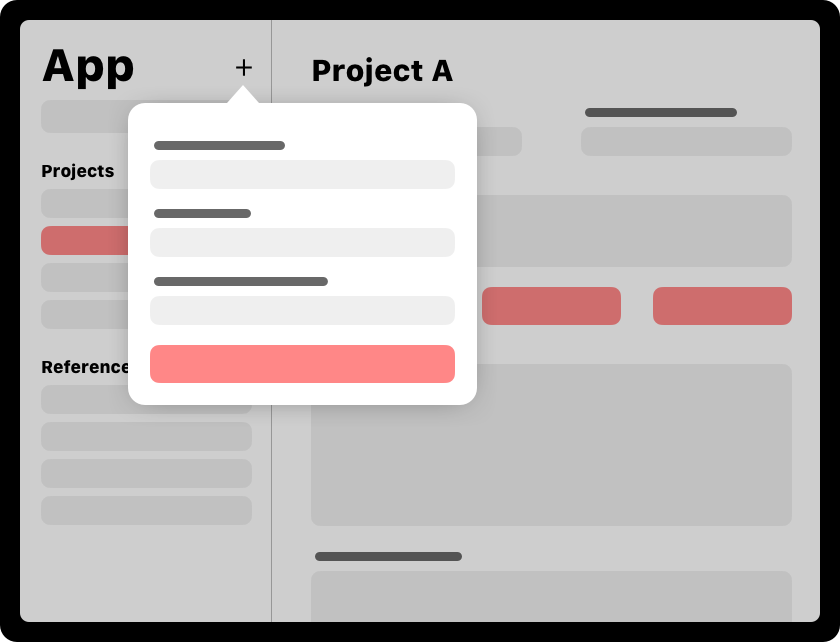
\includegraphics[scale=0.4]{images/design-project-create}
	\caption{Mockup der Erstellung eines neuen Projektes}
	\label{fig:design-project-create}
\end{figure}
Neben dem geplanten Ablauf der Erstellung eines Projektes muss zusätzlich definiert werden, wie ein Projekt gespeichert wird.
Um das weitergeben von Indoor Architect Projekten möglichst leicht zu halten ist ein Projekt lediglich ein Ordner, welcher eine bestimmte Struktur haben muss.
Die Ordner müssen die Endung \texttt{imdfproj} haben, wie zum Beispiel \texttt{ein-projekt.imdfproj/}.
Innerhalb dieses Ordners muss folgende Struktur eingehalten werden:
\vspace{5pt}
\dirtree{%
	.1 /.
	.2 archive.imdf/.
	.3 address.geojson.
	.3 amenity.geojson.
	.3 ....
	.2 manifest.json.
	.2 overlays/.
	.3 overlay-1/.
	.4 overlay.json.
	.4 overlay.png.
}
\vspace{5pt}
Der Ordner \texttt{archive.imdf/} muss alle Dateien enthalten, die für ein gültiges \acl{imdf} Archiv benötigt werden.
Wenn die Kartendaten eines Projektes bearbeitet werden, dann werden die Koordinaten und Beziehungen in diesen Dateien angepasst.
Obwohl dieser Ordner alle Dateien enthält, handelt es sich nicht um ein gültiges \ac{imdf}-Archiv.
Der Inhalt der \ac{geojson}-Dateien selbst muss nicht ein gültiges \ac{imdf}-Format haben, da auch zusätzliche Informationen in den Dateien hinterlegt werden, die für ein Indoor Architect Projekt nützlich sein können.\pbreak%
%
Das \texttt{overlays/}-Verzeichnis enthält alle verwendeten \emph{Overlays}, die über die Kartendaten gelegt werden können.
Dabei handelt es sich um Grafiken, wie zum Beispiel Grundrisse der Gebäude, die man mit einer Transparenz über die Kartendaten legen kann, um die einzelnen Gebäude und Räume besser nachzeichnen zu können.
Jedes Overlay ist dabei ein eigener Ordner, welcher die zu verwendende Grafik enthält, sowie eine \texttt{overlay.json}, welche die Positionsinformationen zu diesem Overlay speichert.
Im Listing \ref{lst:overlay} wird eine Beispieldarstellung einer \texttt{overlay.json}-Datei gezeigt, in der zum Einen der Dateityp der Grafik hinterlegt wird und zum Anderen die Darstellungsoptionen.
Dabei handelt es sich um die Position, an der die Grafik angezeigt werden soll, sowie die Skalierung und die Rotation der Grafik auf den Kartendaten.
\codelisting{Beispieldarstellung einer \texttt{overlay.json}}{lst:overlay}{json-overlay-example.json}{json}\\
Zu guter Letzt bleibt die \texttt{manifest.json}-Datei, welche die grundlegenden Projektinformationen enthält.
Im folgenden werden die einzelnen Felder des Listings \ref{lst:manifest} genauer erklärt.
\codelisting{Beispieldarstellung einer \texttt{manifest.json} eines Indoor Architect Projektes}{lst:manifest}{json-manifest-example.json}{json}\\
Die \texttt{uuid} identifiziert das Projekt neben allen anderen existierenden Projekten innerhalb der Anwendung.
Neben einfachen Zusatzinformationen, wie dem Titel des Projektes gibt es noch die \texttt{imdfprojVersion}, welche dazu dient die Version des Projektes zu identifizieren.
Falls sich die Projektstruktur verändert kann man anhand dieser Versionsnummer erkennen welche Schritte zum migrieren auf die neue Version nötig sind und die Anwendung kann diese Migration dann selbst übernehmen.
Die Felder \texttt{createdAt} und \texttt{updatedAt} bilden nur Zeitstempel der Erstellung und der letzten Bearbeitung des Projektes ab und die \texttt{session} speichert die Position des Anwenders in den Kartendaten, bevor das Projekt geschlossen wurde.
Das Speichern der Session ermöglicht es der Anwendung beim Nächsten Öffnen des Bearbeitungsmodus der Kartendaten an die Stelle zu springen, an der der Anwender zuvor aufgehört hat.

\section{Bearbeiten der Kartendaten}
Die Bearbeitung der Kartendaten gehört zu den wichtigsten Aufgaben von Indoor Architect.
Um die verschiedenen Feature-Typen des \acl{imdf}s erstellen zu können werden fünf verschiedene Werkzeuge bereitgestellt, von denen drei zum Zeichnen von Elementen gedacht sind.
\begin{description}
\item[Pointer]
Das Pointer-Werkzeug dient als neutrales Werkzeug, mit dem einzelne Elemente ausgewählt werden können beziehungsweise mit ihnen interagiert werden kann.
Neue Elemente lassen sich damit nicht erstellen.
\item[Anchor]
Das Anchor-Werkzeug funktioniert ähnlich wie das Pointer-Werkzeug, nur dass in diesem Fall ein Element, also ein \ac{imdf}-Feature erzeugt wird.
Beim ersten Erstellen wird ein \emph{Anchor}-Feature erstellt, welches im Anschluss bearbeitet werden kann.
\item[Line]
Das Line-Werkzeug dient dazu Linien zu zeichnen, die als anschließendes Feature gespeichert werden können.
Beim erstmaligen Erstellen einer Linie wird diese als \emph{Opening}-Feature erstellt.
\item[Polygon]
Analog zum Line-Werkzeug werden mit dem Polygon-Werkzeug Linien gezeichnet.
Nach dem Abschluss des Zeichnens werden diese Linien geschlossen und als Polygon hinterlegt.
Beim ersten Erstellen eines Polygons wird dieses als \emph{Unit}-Feature hinterlegt und kann auch im Anschluss bearbeitet werden.
\item[Ruler]
Das Ruler-Werkzeug dient lediglich dazu Abstände besser visualisieren zu können.
Wenn dieses Werkzeug aktiviert ist, kann der Abstand zwischen zwei Punkten in Metern angezeigt werden.
\end{description}
Die Werkzeuge können über die Werkzeugleiste auf der linken Seite der Ansicht, welche in der Abbildung \ref{fig:design-map-edit} zu erkennen ist, gewechselt werden.
Wenn mit dem Pointer-Werkzeug auf ein Element geklickt wird, können die Eigenschaften des Features in dem sich öffnenden Popover bearbeitet werden.
\begin{figure}[h!]
	\centering
	\vspace{15pt}
	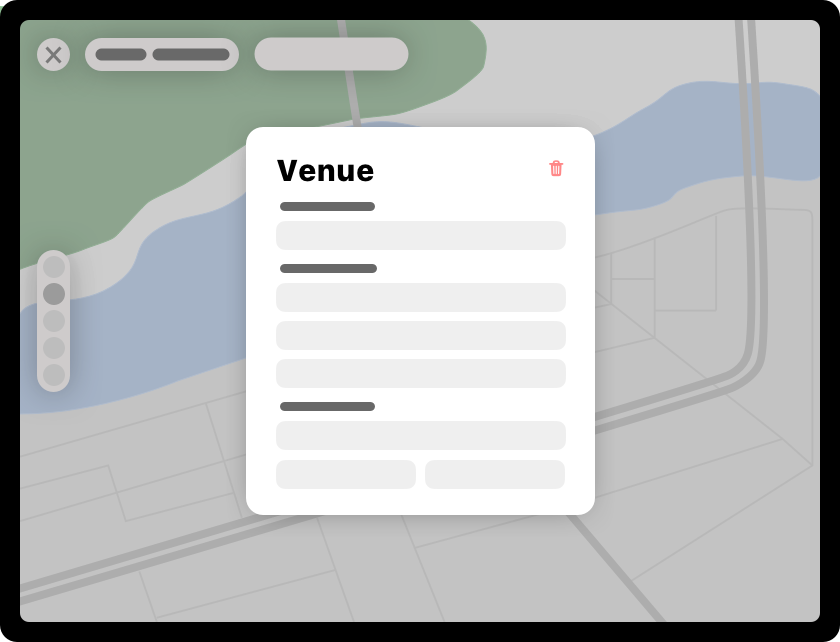
\includegraphics[scale=0.4]{images/design-map-edit}
	\caption{Mockup der Bearbeitung eines Features in der Kartenansicht}
	\label{fig:design-map-edit}
\end{figure}
In der oberen Leiste werden weitere Informationen angezeigt, wie zum Beispiel die Koordinaten des letzten angeklickten Punktes oder das ausgewählte Werkzeug.

\section{Ausführen eines Audits}
\label{sec:validation}
Nach dem Erstellen der Kartendaten soll es möglich sein einen Audit durchzuführen, welcher Rückmeldung darüber gibt, ob die Kartendaten valide sind.
Neben leicht zu identifizierenden Fehlern in der Formalität der gespeicherten Daten, wie ein Fehlender Projekttitel oder eine referenzierte UUID, welche nicht existiert gibt es auch viele semantische Fehler die auftreten können.
Das \acl{imdf} definiert eine große Menge an \emph{Validation Rules}\footnote{\url{https://register.apple.com/resources/imdf/Validations/}. Abruf: 22.08.2020}, welche erfolgreich sein müssen, damit es sich um ein valides \ac{imdf} handelt.
Darunter fallen unter anderem Regeln wie \texttt{AddressMustHaveLocality}, mit welcher validiert wird, dass eine hinterlegte Adresse auch immer eine angegebene Stadt hat, oder auch \texttt{AnchorMustBeWithinReferencedUnit}, womit validiert wird, dass ein gesetzter Anchor mit einer Referenz zu einer bestimmten Unit auch immer innerhalb dieser Unit sein muss.
\begin{figure}[h!]
	\centering
	\vspace{15pt}
	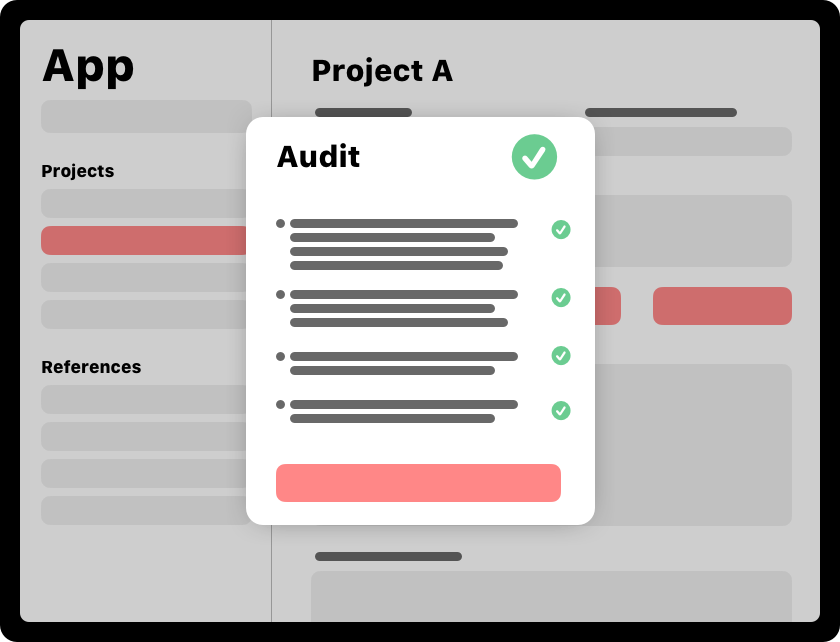
\includegraphics[scale=0.4]{images/design-project-audit}
	\caption{Mockup der Ausführung eines Projektaudits}
	\label{fig:design-project-audit}
\end{figure}
Der Audit sollte die Fehler in den Kartendaten erkennen und dem Anwender aufzeigen (siehe Abbildung \ref{fig:design-project-audit}).
Wenn Warnungen oder gar Fehler auftreten, sollten Lösungen vorgeschlagen werden und nach Möglichkeit die Fehler automatisch behoben werden.

\section{Exportieren der Projekte}
Nach dem erfolgreichen Validieren der Kartendaten steht in der Regel der Export in ein \ac{imdf}-Archiv an.
Da die Kartendaten in dem Indoor Architect Projekt selbst in der \ac{imdf}-Struktur hinterlegt sind besteht ein Export grundlegend nur aus dem archivieren der Daten und dem Speichern an einem gewählten Speicherort.
Das exportierte ZIP-Archiv kann im Anschluss für eine beliebige Verwendung weitergegeben werden.\pbreak%
%
Neben dem Export als \ac{imdf}-Archiv sollte auch ein Export als Indoor Architect Projekt möglich sein.
Das Projekt enthält Zusatzinformationen zu allen Features und Overlays, die an verschiedenen Stellen auf den Kartendaten positioniert sind.
Diese Informationen sind notwendig, wenn das eigene Projekt auf einem anderen Gerät weitergeführt werden soll.
